\renewcommand{\thesection}{\arabic{section}}\renewcommand{\theHsection}{chapter.\arabic{section}}\setcounter{section}{9}\section{多重积分}
\noindent\begin{minipage}{\textwidth}\ProblemHeading{例题}{10.1（改写）}
设 $I=[a,b]\times[c,d]$，$f$ 在 $I$ 上恒取常数值 $k$。由二重积分的定义证明 $f$ 在 $I$ 上可积，并求 $\int_I f\,d\sigma$。
\end{minipage}\par\vfill
\noindent\begin{minipage}{\textwidth}\ProblemHeading{例题}{10.2（改写）}
定义 $D(x,y)=1$（$x,y$ 均为有理数时），其余点取 $D(x,y)=0$。证明 $D$ 在任意面积为正的闭矩形 $I\subset\mathbb R^2$ 上都不可积，并求它的 Darboux 上、下积分。
\end{minipage}\par\vfill
\noindent\begin{minipage}{\textwidth}\ProblemHeading{习题}{10.3}
设一元函数 $f,g$ 在 $[0,1]$ 上 Riemann 可积。证明二元函数 $f(x)g(y)$ 在 $I=[0,1]^2$ 上可积，且\[\iint_I f(x)g(y)\,dx\,dy=\left(\int_0^1f(x)\,dx\right)\left(\int_0^1g(y)\,dy\right).\]
\end{minipage}\par\vfill
\newpage
\noindent\begin{minipage}{\textwidth}\ProblemHeading{习题}{10.4}
计算积分 $\displaystyle\iint_{[0,1]\times[0,1]}e^{x+y}\,dx\,dy$。
\end{minipage}\par\vfill
\noindent\begin{minipage}{\textwidth}\ProblemHeading{习题}{10.5}
设 $a>0$，$I=[-a,a]\times[-a,a]$。证明 $\iint_I\sin(x+y)\,dx\,dy=0$，并从几何上说明这一结果。
\end{minipage}\par\vfill
\noindent\begin{minipage}{\textwidth}\ProblemHeading{习题}{10.6}
设 $f$ 在闭矩形 $I=[a,b]\times[c,d]$ 上有界。对矩形分割 $\pi=\{I_1,\ldots,I_k\}$，记 $\|\pi\|=\max_i\operatorname{diam}(I_i)$、$M_i=\sup_{I_i}f$、$m_i=\inf_{I_i}f$、$\omega_i=M_i-m_i$，并记 $\overline S(f,\pi)=\sum_iM_i\sigma(I_i)$、$\underline S(f,\pi)=\sum_im_i\sigma(I_i)$。证明下列四个条件等价：$f$ 在 $I$ 上 Riemann 可积；$\lim_{\|\pi\|\to0}\sum_i\omega_i\sigma(I_i)=0$；对每个 $\varepsilon>0$，存在分割 $\pi$ 使 $\overline S(f,\pi)-\underline S(f,\pi)<\varepsilon$；$f$ 的 Darboux 上积分与下积分相等。
\end{minipage}\par\vfill
\newpage
\noindent\begin{minipage}{\textwidth}\ProblemHeading{习题}{10.7}
证明：闭矩形上的连续函数 Riemann 可积。
\end{minipage}\par\vfill
\noindent\begin{minipage}{\textwidth}\ProblemHeading{例题}{10.8}
设 $B\subset\mathbb R^2$ 是参数曲线 $\gamma(t)=(x(t),y(t))$（$\alpha\le t\le\beta$）的像，$x,y$ 连续，且其中至少一个分量具有连续导数。证明 $B$ 是 Jordan 零面积集。
\end{minipage}\par\vfill
\noindent\begin{minipage}{\textwidth}\ProblemHeading{例题}{10.9（改写）}
设 $f:[a,b]\to\mathbb R$ 连续。证明其图像 $G(f)=\{(x,f(x)):x\in[a,b]\}$ 是 Jordan 零面积集。
\end{minipage}\par\vfill
\newpage
\noindent\begin{minipage}{\textwidth}\ProblemHeading{例题}{10.10（改写）}
设平面参数曲线 $\gamma(t)=(x(t),y(t))$（$\alpha\le t\le\beta$）为光滑曲线段，即 $x^{\prime},y^{\prime}$ 连续且 $x^{\prime}(t)^2+y^{\prime}(t)^2>0$。证明它是 Jordan 零面积集。
\end{minipage}\par\vfill
\noindent\begin{minipage}{\textwidth}\ProblemHeading{习题}{10.11}
设 $B\subset\mathbb R^2$，$f:B\to\mathbb R$ 有界。对 $x\in B$、$r>0$，令 $I_{x,r}=B\cap B_r(x)$，并以 $\omega_f(x,r)=\sup_{I_{x,r}}f-\inf_{I_{x,r}}f$ 表示 $f$ 在此集合上的振幅。证明\[\omega_f(x,r)=\sup\{|f(y_1)-f(y_2)|:y_1,y_2\in I_{x,r}\}.\]
\end{minipage}\par\vfill
\noindent\begin{minipage}{\textwidth}\ProblemHeading{例题}{10.12}
设 $f(x,y)=\sin\!\bigl(1/((1-x^2)^2+(1-y^2)^2)\bigr)$。在该式未定义的四个点任意补充有限函数值，证明 $f$ 在矩形 $[-2,2]\times[-2,2]$ 上 Riemann 可积。
\end{minipage}\par\vfill
\newpage
\noindent\begin{minipage}{\textwidth}\ProblemHeading{例题}{10.13}
设 $f(x,y)=\arctan\!\bigl(1/(y-x^2)\bigr)$。在抛物线段 $y=x^2$ 上补充函数值，使 $f$ 在 $[0,1]^2$ 上保持有界。证明补充后的 $f$ 在此矩形上 Riemann 可积。
\end{minipage}\par\vfill
\noindent\begin{minipage}{\textwidth}\ProblemHeading{习题}{10.14}
设点列 $\{p_n\}$ 在 $\mathbb R^2$ 中收敛。证明点集 $B=\{p_n:n\ge1\}$ 是 Jordan 零面积集。
\end{minipage}\par\vfill
\noindent\begin{minipage}{\textwidth}\ProblemHeading{习题}{10.15}
设有界集 $B\subset\mathbb R^2$，且其导集 $B^{\prime}$ 是 Jordan 零面积集。证明 $\overline B$ 也是 Jordan 零面积集。
\end{minipage}\par\vfill
\newpage
\noindent\begin{minipage}{\textwidth}\ProblemHeading{习题}{10.16}
证明：$[0,1]^2$ 中所有两个坐标均为有理数的点组成的集合是 Lebesgue 零测集，但不是 Jordan 零面积集。
\end{minipage}\par\vfill
\noindent\begin{minipage}{\textwidth}\ProblemHeading{习题}{10.17}
设闭矩形 $J\subset I$，$f$ 在 $I$ 上 Riemann 可积。证明 $f$ 在 $J$ 上也可积。
\end{minipage}\par\vfill
\noindent\begin{minipage}{\textwidth}\ProblemHeading{习题}{10.18}
设 $I$ 为面积为正的闭矩形，$f$ 在 $I$ 上 Riemann 可积且处处严格大于零。证明 $\int_I f\,d\sigma>0$。
\end{minipage}\par\vfill
\newpage
\noindent\begin{minipage}{\textwidth}\ProblemHeading{习题}{10.19}
研究函数 $f:[0,1]^2\to\mathbb R$ 的 Riemann 可积性，其中\[f(x,y)=\begin{cases}\sin\dfrac1{xy},&x\ne0\text{ 且 }y\ne0,\\0,&x=0\text{ 或 }y=0.\end{cases}\]
\end{minipage}\par\vfill
\noindent\begin{minipage}{\textwidth}\ProblemHeading{习题}{10.20}
设 $I$ 为有界闭矩形，$B=\{p_1,p_2,\ldots\}\subset I$，其中 $p_n$ 两两不同。定义 $f(p_n)=1/n$（$n\ge1$），在 $I\setminus B$ 上令 $f=0$。研究 $f$ 在 $I$ 上的 Riemann 可积性。
\end{minipage}\par\vfill
\noindent\begin{minipage}{\textwidth}\ProblemHeading{习题}{10.21}
设 $f,g$ 在闭矩形 $I$ 上 Riemann 可积。证明 $fg$ 在 $I$ 上可积；若 $g$ 在 $I$ 上处处非零且 $f/g$ 有界，再证明 $f/g$ 在 $I$ 上可积。
\end{minipage}\par\vfill
\newpage
\noindent\begin{minipage}{\textwidth}\ProblemHeading{习题}{10.22}
设 $f$ 在闭矩形 $I$ 上 Riemann 可积。证明 $|f|$ 也可积，且 $\left|\int_I f\,d\sigma\right|\le\int_I|f|\,d\sigma$。
\end{minipage}\par\vfill
\noindent\begin{minipage}{\textwidth}\ProblemHeading{习题}{10.23}
设 $f$ 在闭矩形 $I$ 上 Riemann 可积，且 $\int_I f\,d\sigma>0$。证明存在面积为正的闭矩形 $J\subset I$，使 $f$ 在 $J$ 上处处严格大于零。
\end{minipage}\par\vfill
\noindent\begin{minipage}{\textwidth}\ProblemHeading{习题}{10.24（校订）}
对 $(x,y)\in[0,1]^2$ 定义函数：当 $x=n/m$、$y=p/q$ 为正有理数，且分数均既约、分母为正时，令 $f(x,y)=1/m+1/q$；其余情形令 $f(x,y)=0$。证明 $f$ 在 $[0,1]^2$ 上 Riemann 可积。
\end{minipage}\par\vfill
\newpage
\noindent\begin{minipage}{\textwidth}\ProblemHeading{例题}{10.25}
设 $I=[0,\pi]\times[0,1]$。计算二重积分 $\iint_I y\sin(xy)\,dx\,dy$。
\end{minipage}\par\vfill
\noindent\begin{minipage}{\textwidth}\ProblemHeading{例题}{10.26}
计算二重积分 $\displaystyle\iint_{[0,1]^2}xy^3e^{x^2+y^2}\,dx\,dy$。
\end{minipage}\par\vfill
\noindent\begin{minipage}{\textwidth}\ProblemHeading{例题}{10.27}
在 $I=[0,1]^2$ 上，令 $f(x,y)=1-x-y$（$x+y\le1$），$f(x,y)=0$（$x+y>1$）。计算 $\int_I f\,d\sigma$。
\end{minipage}\par\vfill
\newpage
\noindent\begin{minipage}{\textwidth}\ProblemHeading{例题}{10.28（改写）}
设 $p\ge1$。已知对 $[a,b]\times[c,d]$ 上的非负连续函数 $F$，积分形式的 Minkowski 不等式为\[\left\|\int_c^d F(\cdot,y)\,dy\right\|_p\le \int_c^d \big\|F(\cdot,y)\big\|_p\,dy,\qquad \|u\|_p=\left(\int_a^b |u(x)|^p\,dx\right)^{1/p}.\]由此证明：若 $h,g$ 在 $[a,b]$ 上非负连续，则 $\|h+g\|_p\le \|h\|_p+\|g\|_p$。
\end{minipage}\par\vfill
\noindent\begin{minipage}{\textwidth}\ProblemHeading{习题}{10.29}
计算下列积分。
\SubQ{1}{$\displaystyle\iint_I\frac{x^2}{1+y^2}\,dx\,dy$，$I=[0,1]^2$。}
\SubQ{2}{$\displaystyle\iint_I x\cos(xy)\,dx\,dy$，$I=[0,\pi/2]\times[0,1]$。}
\SubQ{3}{$\displaystyle\iint_I\sin(x+y)\,dx\,dy$，$I=[0,\pi]^2$。}
\end{minipage}\par\vfill
\noindent\begin{minipage}{\textwidth}\ProblemHeading{习题}{10.30}
设 $f$ 在矩形 $I=[a,b]\times[c,d]$ 上具有连续的二阶偏导数。计算 $\iint_I\frac{\partial^2f}{\partial x\partial y}(x,y)\,dx\,dy$。
\end{minipage}\par\vfill
\newpage
\noindent\begin{minipage}{\textwidth}\ProblemHeading{习题}{10.31}
计算 $\int_I f\,d\sigma$，其中 $I=[0,1]^2$，$f$ 分别如下。
\SubQ{1}{$f(x,y)=1$（$y\le x^2$），$f(x,y)=0$（$y>x^2$）。}
\SubQ{2}{$f(x,y)=x+y$（$x^2\le y\le2x^2$），其余点取 $f(x,y)=0$。}
\end{minipage}\par\vfill
\noindent\begin{minipage}{\textwidth}\ProblemHeading{习题}{10.32}
利用积分形式的 Minkowski 不等式\[\left(\int_a^b\left(\int_c^dF(x,y)\,dy\right)^pdx\right)^{1/p}\le\int_c^d\left(\int_a^bF(x,y)^p\,dx\right)^{1/p}dy,\]证明：对 $a_k,b_k\ge0$（$1\le k\le n$）、$p\ge1$，有\[\left(\sum_{k=1}^n(a_k+b_k)^p\right)^{1/p}\le\left(\sum_{k=1}^na_k^p\right)^{1/p}+\left(\sum_{k=1}^nb_k^p\right)^{1/p}.\]
\end{minipage}\par\vfill
\noindent\begin{minipage}{\textwidth}\ProblemHeading{习题}{10.33}
设 $f,g$ 均在 $[a,b]$ 上可积。利用\[\iint_{[a,b]^2}(f(x)g(y)-f(y)g(x))^2\,dx\,dy\ge0,\]证明 Cauchy--Schwarz 不等式\[\left(\int_a^bf(x)g(x)\,dx\right)^2\le\left(\int_a^bf(x)^2\,dx\right)\left(\int_a^bg(x)^2\,dx\right).\]
\end{minipage}\par\vfill
\newpage
\noindent\begin{minipage}{\textwidth}\ProblemHeading{习题}{10.34}
在 $[0,1]^2$ 上定义 $f(x,y)=1/m+1/q$，当 $x=n/m$、$y=p/q$ 为既约的正有理数时；其余点取 $f=0$。证明：固定正有理数 $p/q\in[0,1]$ 时，$f(x,p/q)$ 关于 $x$ 不 Riemann 可积；固定正有理数 $n/m\in[0,1]$ 时，$f(n/m,y)$ 关于 $y$ 不 Riemann 可积。
\end{minipage}\par\vfill
\noindent\begin{minipage}{\textwidth}\ProblemHeading{习题}{10.35（校订）}
对 $(x,y)\in[0,1]^2$，当 $x=n/m$、$y=p/m$ 为既约的正有理数且最简分母相同时，令 $g(x,y)=1$；其余点令 $g(x,y)=0$。证明两个累次积分\[\int_0^1dx\int_0^1g(x,y)\,dy,\qquad\int_0^1dy\int_0^1g(x,y)\,dx\]都存在，但 $g$ 在 $[0,1]^2$ 上不 Riemann 可积。
\end{minipage}\par\vfill
\noindent\begin{minipage}{\textwidth}\ProblemHeading{例题}{10.36（改写）}
设 $B=([0,1]\cap\mathbb Q)^2$，并令 $f:B\to\mathbb R$ 恒等于零。将 $f$ 在 $B$ 外延拓为零，按此延拓定义 $f$ 在 $B$ 上的 Riemann 积分。证明 $f$ 在 $B$ 上可积，并求 $\partial B$，说明 $f$ 可积并不要求 $B$ 的边界为 Lebesgue 零测集。
\end{minipage}\par\vfill
\newpage
\noindent\begin{minipage}{\textwidth}\ProblemHeading{习题}{10.37}
设有界集 $B\subset\mathbb R^2$，$f:B\to\mathbb R$ 在 $B$ 上 Riemann 可积。证明任意常数 $c$ 都使 $cf$ 在 $B$ 上可积，且 $\int_B cf\,d\sigma=c\int_B f\,d\sigma$。
\end{minipage}\par\vfill
\noindent\begin{minipage}{\textwidth}\ProblemHeading{习题}{10.38}
设 $B\subset\mathbb R^2$ 有界。证明 $B$ 有 Jordan 面积当且仅当其边界 $\partial B$ 是 Jordan 零面积集。
\end{minipage}\par\vfill
\noindent\begin{minipage}{\textwidth}\ProblemHeading{习题}{10.39}
证明\[1.96<\iint_{|x|+|y|\le10}\frac{dx\,dy}{100+\cos^2x+\cos^2y}<2.\]
\end{minipage}\par\vfill
\newpage
\noindent\begin{minipage}{\textwidth}\ProblemHeading{习题}{10.40}
设 $B\subset\mathbb R^2$ 有界。证明 $B$ 有 Jordan 面积的充要条件是：对任意满足 $I^\circ\supset B$ 的闭矩形 $I$ 及其矩形网格分割 $\pi=\{I_j\}$，均有\[\lim_{\|\pi\|\to0}\sum_{I_j\cap B\ne\varnothing}\sigma(I_j)=\lim_{\|\pi\|\to0}\sum_{I_j\subset B}\sigma(I_j).\]
\end{minipage}\par\vfill
\noindent\begin{minipage}{\textwidth}\ProblemHeading{例题}{10.41}
设 $a,b>0$，$B$ 为图中所围成的三角形。计算 $\iint_Bx^2y^2\,dx\,dy$。
\begin{center}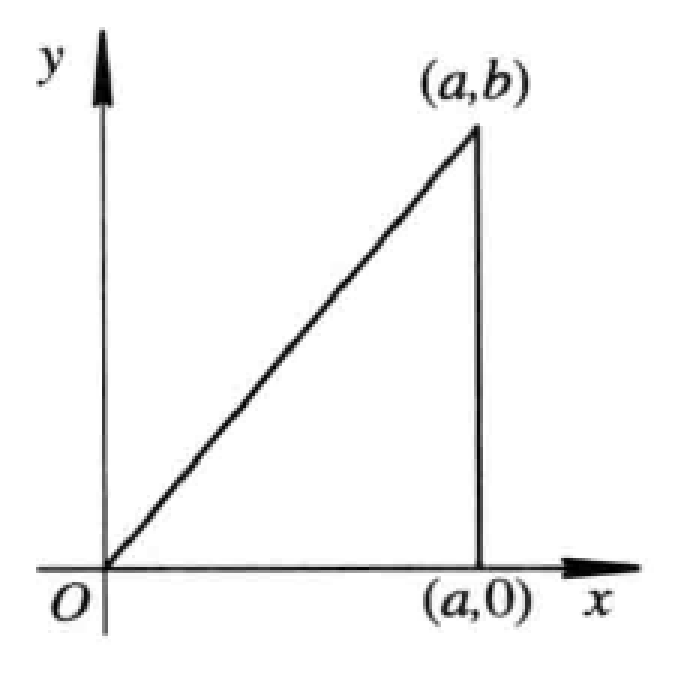
\includegraphics[width=0.28\linewidth]{figures/fig_10_41_1.png}\end{center}
\end{minipage}\par\vfill
\noindent\begin{minipage}{\textwidth}\ProblemHeading{例题}{10.42}
设 $B$ 为两组平行直线 $y=a,y=3a$ 与 $y=x,y=x+a$ 围成的平行四边形（$a\ne0$）。计算 $\iint_B(x^2+y^2)\,dx\,dy$。
\end{minipage}\par\vfill
\newpage
\noindent\begin{minipage}{\textwidth}\ProblemHeading{例题}{10.43}
设 $B=\{(x,y):|x|+|y|\le1\}$。计算 $\iint_Bxy^2\,dx\,dy$。
\end{minipage}\par\vfill
\noindent\begin{minipage}{\textwidth}\ProblemHeading{例题}{10.44}
计算累次积分 $\displaystyle\int_0^1dy\int_y^{\sqrt y}\frac{\sin x}{x}\,dx$。
\end{minipage}\par\vfill
\noindent\begin{minipage}{\textwidth}\ProblemHeading{例题}{10.45}
计算两个圆柱体 $x^2+y^2\le a^2$ 与 $x^2+z^2\le a^2$ 相交所成的立体体积，其中 $a>0$。
\end{minipage}\par\vfill
\newpage
\noindent\begin{minipage}{\textwidth}\ProblemHeading{习题}{10.46}
计算下列积分，其中出现的参数 $a>0$，$\lfloor t\rfloor$ 表示不超过 $t$ 的最大整数。
\SubQ{1}{$\displaystyle\iint_D\cos(x+y)\,dx\,dy$，$D$ 由 $x=0,y=x,y=\pi$ 围成。}
\SubQ{2}{$\displaystyle\iint_Dxy^2\,dx\,dy$，$D$ 由 $y^2=4x$ 与 $x=1$ 围成。}
\SubQ{3}{$\displaystyle\iint_De^{x+y}\,dx\,dy$，$D=\{(x,y):|x|+|y|\le1\}$。}
\end{minipage}\par\vfill
\noindent\begin{minipage}{\textwidth}\ProblemHeading{习题}{10.47}
计算下列积分，其中出现的参数 $a>0$，$\lfloor t\rfloor$ 表示不超过 $t$ 的最大整数。
\SubQ{1}{$\displaystyle\iint_D|xy|\,dx\,dy$，$D=\{(x,y):x^2+y^2\le a^2\}$。}
\SubQ{2}{$\displaystyle\iint_Dx\cos(xy)\,dx\,dy$，$D=\{(x,y):x^2+y^2\le a^2\}$。}
\SubQ{3}{$\displaystyle\iint_D|\cos(x+y)|\,dx\,dy$，$D=[0,1]^2$。}
\end{minipage}\par\vfill
\noindent\begin{minipage}{\textwidth}\ProblemHeading{习题}{10.48}
计算下列积分，其中出现的参数 $a>0$，$\lfloor t\rfloor$ 表示不超过 $t$ 的最大整数。
\SubQ{1}{$\displaystyle\iint_Dy^2\,dx\,dy$，$D$ 由旋轮线 $x=a(t-\sin t),y=a(1-\cos t)$（$0\le t\le2\pi$）与 $y=0$ 围成。}
\SubQ{2}{$\displaystyle\iint_D\lfloor x+y\rfloor\,dx\,dy$，$D=[0,2]^2$。}
\end{minipage}\par\vfill
\newpage
\noindent\begin{minipage}{\textwidth}\ProblemHeading{习题}{10.49}
改变下列累次积分的积分次序。
\SubQ{1}{$\displaystyle\int_0^1dx\int_0^{x^2}f(x,y)\,dy$。}
\SubQ{2}{$\displaystyle\int_1^e dx\int_0^{\ln x}f(x,y)\,dy$。}
\SubQ{3}{$\displaystyle\int_0^1dx\int_{x^2}^{x}f(x,y)\,dy$。}
\end{minipage}\par\vfill
\noindent\begin{minipage}{\textwidth}\ProblemHeading{习题}{10.50}
改变下列累次积分的积分次序。
\SubQ{1}{$\displaystyle\int_a^b dx\int_a^x f(x,y)\,dy$（$a<b$）。}
\SubQ{2}{$\displaystyle\int_{-1}^1dx\int_{-\sqrt{1-x^2}}^{1-x^2}f(x,y)\,dy$。}
\SubQ{3}{$\displaystyle\int_0^1dx\int_{x-1}^{1-x}f(x,y)\,dy$。}
\end{minipage}\par\vfill
\noindent\begin{minipage}{\textwidth}\ProblemHeading{习题}{10.51}
改变下列累次积分的积分次序。
\SubQ{1}{$\displaystyle\int_0^\pi dx\int_0^{\cos x}f(x,y)\,dy$。}
\end{minipage}\par\vfill
\newpage
\noindent\begin{minipage}{\textwidth}\ProblemHeading{习题}{10.52}
设 $f$ 为一元连续函数，$a>0$。证明\[\int_0^a dx\int_0^x f(x)f(y)\,dy=\frac12\left(\int_0^af(t)\,dt\right)^2.\]
\end{minipage}\par\vfill
\noindent\begin{minipage}{\textwidth}\ProblemHeading{习题}{10.53}
设 $f$ 连续，$a>0$。证明 $\int_0^a dx\int_0^xf(y)\,dy=\int_0^a(a-t)f(t)\,dt$。
\end{minipage}\par\vfill
\noindent\begin{minipage}{\textwidth}\ProblemHeading{习题}{10.54}
设 $a<b$，$f$ 连续。证明\[\int_a^b dx\int_a^xdy\int_a^yf(x,y,z)\,dz=\int_a^b dz\int_z^bdy\int_y^bf(x,y,z)\,dx.\]
\end{minipage}\par\vfill
\newpage
\noindent\begin{minipage}{\textwidth}\ProblemHeading{习题}{10.55}
设 $f$ 连续，$a>0$。证明\[\int_0^a dx\int_0^xdy\int_0^yf(x)f(y)f(z)\,dz=\frac1{3!}\left(\int_0^af(t)\,dt\right)^3.\]
\end{minipage}\par\vfill
\noindent\begin{minipage}{\textwidth}\ProblemHeading{习题}{10.56}
设 $f$ 连续，$a>0$。证明\[\int_0^a dx\int_0^xdy\int_0^yf(z)\,dz=\frac12\int_0^a(a-t)^2f(t)\,dt.\]
\end{minipage}\par\vfill
\noindent\begin{minipage}{\textwidth}\ProblemHeading{习题}{10.57}
设 $f$ 在原点邻域内连续。求极限 $\displaystyle\lim_{r\to0}\frac1{\pi r^2}\iint_{x^2+y^2\le r^2}f(x,y)\,dx\,dy$。
\end{minipage}\par\vfill
\newpage
\noindent\begin{minipage}{\textwidth}\ProblemHeading{例题}{10.58}
设 $0<p<q$、$0<a<b$，$D$ 为第一象限中由四条抛物线 $y^2=px,y^2=qx,x^2=ay,x^2=by$ 围成的曲边四边形。计算 $D$ 的面积及 $\iint_D\frac1{xy}\,dx\,dy$。
\end{minipage}\par\vfill
\noindent\begin{minipage}{\textwidth}\ProblemHeading{例题}{10.59}
设 $D=\{(x,y):x\ge0,y\ge0,x+y\le1\}$。计算 $\displaystyle\iint_D\exp\!\left(\frac{x-y}{x+y}\right)\,dx\,dy$，原点处可任意补充有限函数值。
\end{minipage}\par\vfill
\noindent\begin{minipage}{\textwidth}\ProblemHeading{例题}{10.60}
设 $a>0$。球体 $x^2+y^2+z^2\le a^2$ 被柱面 $x^2+y^2=ax$ 所截，求柱面内部与球体相交部分的体积。
\end{minipage}\par\vfill
\newpage
\noindent\begin{minipage}{\textwidth}\ProblemHeading{例题}{10.61}
设 $a,b>0$。用二重积分求椭圆 $x^2/a^2+y^2/b^2=1$ 所围图形的面积。
\end{minipage}\par\vfill
\noindent\begin{minipage}{\textwidth}\ProblemHeading{例题}{10.62}
计算反常积分 $\displaystyle\int_0^{+\infty}e^{-x^2}\,dx$。
\end{minipage}\par\vfill
\noindent\begin{minipage}{\textwidth}\ProblemHeading{习题}{10.63}
计算下列二重积分。
\SubQ{1}{$\displaystyle\iint_D(x-y)^2\sin(x+y)\,dx\,dy$，$D$ 为顶点 $(\pi,0),(2\pi,\pi),(\pi,2\pi),(0,\pi)$ 顺次连接成的正方形。}
\SubQ{2}{$\displaystyle\iint_D(x^2+y^2)\,dx\,dy$，$D$ 是第一象限中由 $x^2-y^2=1,x^2-y^2=2,xy=1,xy=2$ 围成的图形。}
\end{minipage}\par\vfill
\newpage
\noindent\begin{minipage}{\textwidth}\ProblemHeading{习题}{10.64}
计算下列曲线围成的图形的面积。
\SubQ{1}{$(a_1x+b_1y+c_1)^2+(a_2x+b_2y+c_2)^2=1$，其中 $a_1b_2\ne a_2b_1$。}
\SubQ{2}{$\sqrt x+\sqrt y=\sqrt a$、$x=0$、$y=0$，其中 $a>0$。}
\end{minipage}\par\vfill
\noindent\begin{minipage}{\textwidth}\ProblemHeading{习题}{10.65}
设 $f$ 连续。证明\[\iint_{|x|+|y|\le1}f(x+y)\,dx\,dy=\int_{-1}^1f(t)\,dt.\]
\end{minipage}\par\vfill
\noindent\begin{minipage}{\textwidth}\ProblemHeading{习题}{10.66}
设 $f$ 连续，$D$ 为第一象限中由 $xy=1,xy=2,y=x,y=4x$ 围成的图形。证明\[\iint_Df(xy)\,dx\,dy=\ln2\int_1^2f(t)\,dt.\]
\end{minipage}\par\vfill
\newpage
\noindent\begin{minipage}{\textwidth}\ProblemHeading{习题}{10.67}
计算下列二重积分，其中 $R>0$。
\SubQ{1}{$\displaystyle\iint_{\pi^2\le x^2+y^2\le4\pi^2}\sin\sqrt{x^2+y^2}\,dx\,dy$。}
\SubQ{2}{$\displaystyle\iint_{x^2+y^2\le Rx}\sqrt{R^2-x^2-y^2}\,dx\,dy$。}
\SubQ{3}{$\displaystyle\iint_{\substack{x^2+y^2\le1\\x\le0,\ y\le0}}\arctan\frac yx\,dx\,dy$（在坐标轴上的未定义点任意补充有限函数值）。}
\end{minipage}\par\vfill
\noindent\begin{minipage}{\textwidth}\ProblemHeading{习题}{10.68}
计算下列二重积分，其中 $R>0$。
\SubQ{1}{$\displaystyle\iint_{x^2+y^2\le x+y}\sqrt{x^2+y^2}\,dx\,dy$。}
\end{minipage}\par\vfill
\noindent\begin{minipage}{\textwidth}\ProblemHeading{习题}{10.69}
计算半径为 $R>0$ 的球的体积。
\end{minipage}\par\vfill
\newpage
\noindent\begin{minipage}{\textwidth}\ProblemHeading{习题}{10.70}
设 $a,b>0$，$D=\{(x,y):x^2/a^2+y^2/b^2\le1,\ x\ge y\ge0\}$。计算\[\iint_D\sqrt{\frac{x^2}{a^2}+\frac{y^2}{b^2}}\,dx\,dy.\]
\end{minipage}\par\vfill
\noindent\begin{minipage}{\textwidth}\ProblemHeading{习题}{10.71}
证明 $\displaystyle\iint_{[0,1]^2}(xy)^{xy}\,dx\,dy=\int_0^1t^t\,dt$，在 $xy=0$ 处把被积函数连续补为 $1$。
\end{minipage}\par\vfill
\noindent\begin{minipage}{\textwidth}\ProblemHeading{习题}{10.72}
设常数 $a,b$ 不全为零，$f$ 连续。证明\[\iint_{x^2+y^2\le1}f(ax+by+c)\,dx\,dy=2\int_{-1}^1\sqrt{1-t^2}\,f\!\left(t\sqrt{a^2+b^2}+c\right)\,dt.\]
\end{minipage}\par\vfill
\newpage
\noindent\begin{minipage}{\textwidth}\ProblemHeading{习题}{10.73}
设单变量函数 $f$ 连续可导，$t>0$，令 $F(t)=\iint_{[0,t]^2}f(xy)\,dx\,dy$。证明：
\SubQ{1}{$\displaystyle F^{\prime}(t)=\frac2t\left(F(t)+\iint_{[0,t]^2}xyf^{\prime}(xy)\,dx\,dy\right)$。}
\SubQ{2}{$\displaystyle F^{\prime}(t)=\frac2t\int_0^{t^2}f(s)\,ds$。}
\end{minipage}\par\vfill
\noindent\begin{minipage}{\textwidth}\ProblemHeading{习题}{10.74}
计算 $\displaystyle\iint_D\frac{dx\,dy}{xy(\ln^2x+\ln^2y)}$，其中 $D$ 为第一象限中圆周 $x^2+y^2=1$ 与直线 $x+y=1$ 所围成的图形；积分按内部极限理解。
\end{minipage}\par\vfill
\noindent\begin{minipage}{\textwidth}\ProblemHeading{例题}{10.75}
设 $V=\{(x,y,z):x,y,z\ge0,\ x+y+z\le1\}$。计算\[\iiint_V\frac{dx\,dy\,dz}{(1+x+y+z)^3}.\]
\end{minipage}\par\vfill
\newpage
\noindent\begin{minipage}{\textwidth}\ProblemHeading{习题}{10.76}
设 $\Delta,D\subset\mathbb R^3$ 为有 Jordan 体积的有界闭区域，$\varphi$ 在 $\Delta$ 的邻域内为 $C^1$ 映射，将 $\Delta$ 一一映到 $D$，且 $\det D\varphi\ne0$；$F$ 在 $D$ 上连续。证明三重积分换元公式\[\iiint_DF(x)\,dx=\iiint_\Delta F(\varphi(u))|\det D\varphi(u)|\,du.\]证明中应说明 Jacobi 行列式的绝对值如何给出局部体积的伸缩比。
\end{minipage}\par\vfill
\noindent\begin{minipage}{\textwidth}\ProblemHeading{例题}{10.77}
设 $a>0$，$D$ 为球面 $x^2+y^2+z^2=a^2$ 与锥面 $z=\sqrt{x^2+y^2}$ 所围成的上部立体，即 $x^2+y^2+z^2\le a^2$ 且 $z\ge\sqrt{x^2+y^2}$。计算 $\iiint_D(x^2+y^2+z^2)\,dx\,dy\,dz$。
\end{minipage}\par\vfill
\noindent\begin{minipage}{\textwidth}\ProblemHeading{例题}{10.78}
设 $a>0$，$D$ 为球 $x^2+y^2+z^2\le2az$ 内、球 $x^2+y^2+z^2<az$ 外的部分。计算 $\iiint_Dz\,dx\,dy\,dz$。
\end{minipage}\par\vfill
\newpage
\noindent\begin{minipage}{\textwidth}\ProblemHeading{习题}{10.79}
计算下列三重积分。
\SubQ{1}{$\displaystyle\iiint_Vxyz\,dx\,dy\,dz$，$V=\{x,y,z\ge0:x^2+y^2+z^2\le1\}$。}
\SubQ{2}{$\displaystyle\iiint_V(x+y+z)\,dx\,dy\,dz$，$V$ 为平面 $x+y+z=1$ 与三个坐标平面围成的立体。}
\SubQ{3}{$\displaystyle\iiint_Vxy^2z^3\,dx\,dy\,dz$，$V$ 由 $z=xy,z=0,x=1,x=y$ 围成。}
\end{minipage}\par\vfill
\noindent\begin{minipage}{\textwidth}\ProblemHeading{习题}{10.80}
计算下列曲面围成的有界立体的体积（$a>0$）。
\SubQ{1}{$z^2=x^2+y^2/4$ 与 $2z=x^2+y^2/4$。}
\SubQ{2}{$x^2+z^2=a^2$ 与 $|x|+|y|=a$。}
\end{minipage}\par\vfill
\noindent\begin{minipage}{\textwidth}\ProblemHeading{习题}{10.81}
设 $f$ 在原点邻域连续。求\[\lim_{r\to0^+}\frac3{4\pi r^3}\iiint_{x^2+y^2+z^2\le r^2}f(x,y,z)\,dx\,dy\,dz.\]
\end{minipage}\par\vfill
\newpage
\noindent\begin{minipage}{\textwidth}\ProblemHeading{习题}{10.82}
计算下列三重积分。
\SubQ{1}{$\displaystyle\iiint_{x^2+y^2+z^2\le2}\sqrt{x^2+y^2+z^2}\,dx\,dy\,dz$。}
\SubQ{2}{$\displaystyle\iiint_D(x^2+y^2)\,dx\,dy\,dz$，$D=\{z\ge0:a^2\le x^2+y^2+z^2\le b^2\}$，$0\le a<b$。}
\SubQ{3}{$\displaystyle\iiint_D\sqrt{1-\frac{x^2}{a^2}-\frac{y^2}{b^2}-\frac{z^2}{c^2}}\,dx\,dy\,dz$，$D$ 为椭球 $x^2/a^2+y^2/b^2+z^2/c^2\le1$，$a,b,c>0$。}
\end{minipage}\par\vfill
\noindent\begin{minipage}{\textwidth}\ProblemHeading{习题}{10.83}
计算下列曲面所围成立体的体积。
\SubQ{1}{$a_ix+b_iy+c_iz=\pm h_i$（$i=1,2,3$），其中 $h_i>0$ 且 $\det\!\begin{pmatrix}a_1&b_1&c_1\\a_2&b_2&c_2\\a_3&b_3&c_3\end{pmatrix}\ne0$。}
\SubQ{2}{球面 $x^2+y^2+z^2=a^2$ 与 $x^2+y^2+z^2=b^2$ 之间、$z>0$ 的部分，其中 $0\le a<b$。}
\SubQ{3}{$(x^2+y^2+z^2)^2=a^3z$，其中 $a>0$。}
\end{minipage}\par\vfill
\noindent\begin{minipage}{\textwidth}\ProblemHeading{习题}{10.84}
计算下列曲面所围成立体的体积。
\SubQ{1}{$(x^2+y^2+z^2)^n=z^{2n-1}$，其中 $n\in\mathbb N^*$。}
\SubQ{2}{$\left(x^2/a^2+y^2/b^2+z^2/c^2\right)^2=x^2/a^2+y^2/b^2$，其中 $a,b,c>0$。}
\end{minipage}\par\vfill
\newpage
\noindent\begin{minipage}{\textwidth}\ProblemHeading{习题}{10.85}
设 $f$ 连续可导，$t>0$，令 $F(t)=\iiint_{[0,t]^3}f(xyz)\,dx\,dy\,dz$。证明\[F^{\prime}(t)=\frac3t\left(F(t)+\iiint_{[0,t]^3}xyzf^{\prime}(xyz)\,dx\,dy\,dz\right).\]
\end{minipage}\par\vfill
\noindent\begin{minipage}{\textwidth}\ProblemHeading{习题}{10.86}
设 $f$ 连续，$t>0$，令 $F(t)=\iiint_{[0,t]^3}f(xyz)\,dx\,dy\,dz$、$g(u)=\int_0^uf(s)\,ds$。证明\[F^{\prime}(t)=\frac3t\int_0^{t^3}\frac{g(u)}u\,du.\]
\end{minipage}\par\vfill
\noindent\begin{minipage}{\textwidth}\ProblemHeading{例题}{10.87（改写）}
设 $a>0$、$n\in\mathbb N^*$，$S_n(a)=\{(x_1,\ldots,x_n):x_i\ge0,\ \sum_{i=1}^nx_i\le a\}$。用 $n$ 重积分求 $S_n(a)$ 的体积。
\end{minipage}\par\vfill
\newpage
\noindent\begin{minipage}{\textwidth}\ProblemHeading{例题}{10.88（改写）}
设 $a>0$，$B_n(a)=\{x\in\mathbb R^n:\sum_{i=1}^nx_i^2\le a^2\}$。求 $B_n(a)$ 的 $n$ 维体积，分别给出 $n$ 为偶数和奇数时的表达式。
\end{minipage}\par\vfill
\noindent\begin{minipage}{\textwidth}\ProblemHeading{例题}{10.89（改写）}
设 $n\ge2$。考虑 $n$ 维球坐标变换\[x_j=r\left(\prod_{k=1}^{j-1}\sin\theta_k\right)\cos\theta_j\quad(1\le j\le n-1),\qquad x_n=r\prod_{k=1}^{n-1}\sin\theta_k,\]其中空积为 $1$，$r>0$，$0<\theta_1,\ldots,\theta_{n-2}<\pi$，$0<\theta_{n-1}<2\pi$。计算 Jacobi 行列式 $\dfrac{\partial(x_1,\ldots,x_n)}{\partial(r,\theta_1,\ldots,\theta_{n-1})}$。
\end{minipage}\par\vfill
\noindent\begin{minipage}{\textwidth}\ProblemHeading{例题}{10.90}
设 $a>0$，$f$ 是 $[0,a]$ 上的连续函数，$B_n(a)=\{x\in\mathbb R^n:\sum_{i=1}^nx_i^2\le a^2\}$。把积分\[\int_{B_n(a)}f\!\left(\sqrt{x_1^2+\cdots+x_n^2}\right)\,dx_1\cdots dx_n\]化为一重积分，并明确写出系数。
\end{minipage}\par\vfill
\newpage
\noindent\begin{minipage}{\textwidth}\ProblemHeading{习题}{10.91}
计算下列 $n$ 重积分（$n\in\mathbb N^*$）。
\SubQ{1}{$\displaystyle\int_{[0,1]^n}(x_1^2+\cdots+x_n^2)\,dx_1\cdots dx_n$。}
\SubQ{2}{$\displaystyle\int_{[0,1]^n}(x_1+\cdots+x_n)^2\,dx_1\cdots dx_n$。}
\end{minipage}\par\vfill
\noindent\begin{minipage}{\textwidth}\ProblemHeading{习题}{10.92}
计算累次积分 $\displaystyle\int_0^1dx_1\int_0^{x_1}dx_2\cdots\int_0^{x_{n-1}}x_1\cdots x_n\,dx_n$，其中 $n\in\mathbb N^*$。
\end{minipage}\par\vfill
\noindent\begin{minipage}{\textwidth}\ProblemHeading{习题}{10.93}
计算下列 $\mathbb R^n$ 中区域的体积，其中 $a,a_1,\ldots,a_n>0$。
\SubQ{1}{$V=\{x_i\ge0:\sum_{i=1}^nx_i/a_i\le1\}$。}
\SubQ{2}{$V=\{x\in\mathbb R^n:\sum_{i=1}^n|x_i|\le a\}$。}
\end{minipage}\par\vfill
\newpage
\noindent\begin{minipage}{\textwidth}\ProblemHeading{习题}{10.94}
设 $K$ 是 $[a,b]^2$ 上的连续函数。对 $n\in\mathbb N^*$，定义\[K_n(x,y)=\int_{[a,b]^n}K(x,t_1)K(t_1,t_2)\cdots K(t_n,y)\,dt_1\cdots dt_n.\]证明对 $m,n\in\mathbb N^*$，有 $K_{m+n+1}(x,y)=\int_a^bK_m(x,t)K_n(t,y)\,dt$。
\end{minipage}\par\vfill
\noindent\begin{minipage}{\textwidth}\ProblemHeading{习题}{10.95（校订）}
设 $n\ge2$、$a_1,\ldots,a_n>0$。求区域\[V_n=\left\{x\in\mathbb R^n:\frac{|x_i|}{a_i}+\frac{|x_n|}{a_n}\le1\ (1\le i<n)\right\}\]的体积。
\end{minipage}\par\vfill
\noindent\begin{minipage}{\textwidth}\ProblemHeading{习题}{10.96}
设 $a>0$、$n\in\mathbb N^*$，$f$ 在 $[0,a]$ 上连续。证明\[\int_0^a dx_1\int_0^{x_1}dx_2\cdots\int_0^{x_{n-1}}f(x_n)\,dx_n=\frac1{(n-1)!}\int_0^af(t)(a-t)^{n-1}\,dt.\]
\end{minipage}\par\vfill
\newpage
\noindent\begin{minipage}{\textwidth}\ProblemHeading{习题}{10.97}
设 $a>0$、$n\in\mathbb N^*$，$f$ 在 $[0,a]$ 上连续。证明\[\int_0^a dx_1\int_0^{x_1}dx_2\cdots\int_0^{x_{n-1}}\prod_{i=1}^nf(x_i)\,dx_n=\frac1{n!}\left(\int_0^af(t)\,dt\right)^n.\]
\end{minipage}\par\vfill
\noindent\begin{minipage}{\textwidth}\ProblemHeading{习题}{10.98}
设 $a<b$、$n\in\mathbb N^*$，$f$ 在 $[a,b]^n$ 上连续。证明\[\int_a^b dx_1\int_a^{x_1}dx_2\cdots\int_a^{x_{n-1}}f(x_1,\ldots,x_n)\,dx_n=\int_a^bdx_n\int_{x_n}^bdx_{n-1}\cdots\int_{x_2}^bf(x_1,\ldots,x_n)\,dx_1.\]
\end{minipage}\par\vfill
\noindent\begin{minipage}{\textwidth}\ProblemHeading{例题}{10.99}
一条横截面为半圆形的水渠装满水，水闸为竖直的半圆盘，其半径为 $R$，直径位于水面。设水的重度为常数 $\gamma$（单位体积水的重量）。求水对水闸的总压力。
\end{minipage}\par\vfill
\newpage
\noindent\begin{minipage}{\textwidth}\ProblemHeading{例题}{10.100}
设以原点为中心、半径为 $R>0$ 的球体内物质的密度为 $\rho(p)=a\|p\|$，其中 $a>0$。求球体的总质量。
\end{minipage}\par\vfill
\noindent\begin{minipage}{\textwidth}\ProblemHeading{例题}{10.101}
设球体半径为 $a>0$，球心为 $(0,0,a)$，密度为 $\rho(p)=k/\|p\|^2$（$k>0$）。求该球体的质心；在原点的奇性按反常积分理解。
\end{minipage}\par\vfill
\noindent\begin{minipage}{\textwidth}\ProblemHeading{例题}{10.102}
设均匀球体以原点为中心，半径为 $R>0$，密度为 $1$。取万有引力常数为 $1$，求该球体在空间任意点 $p$ 产生的引力场（即放在 $p$ 处的单位质量质点所受的引力）。分别讨论球内、球面和球外。
\end{minipage}\par\vfill
\newpage
\noindent\begin{minipage}{\textwidth}\ProblemHeading{习题}{10.103}
半径为 $R$ 的均匀圆盘面密度为 $\mu$。过圆心且垂直于圆盘的直线上有一根均匀细棒，线密度为 $\rho$，长度为 $l$，近圆盘一端到圆心的距离为 $a>0$。求圆盘对细棒的引力。设万有引力常数为 $G$。
\end{minipage}\par\vfill
\noindent\begin{minipage}{\textwidth}\ProblemHeading{习题}{10.104}
一正圆锥与一半球体以公共底面相接成均匀球锥，体密度为 $\rho$，公共底面半径为 $R$，圆锥顶角为 $2\alpha$（$0<\alpha<\pi/2$）。设万有引力常数为 $G$，求球锥在圆锥顶点处产生的引力场。
\end{minipage}\par\vfill
